\begin{figure}[ht]
    \centering
    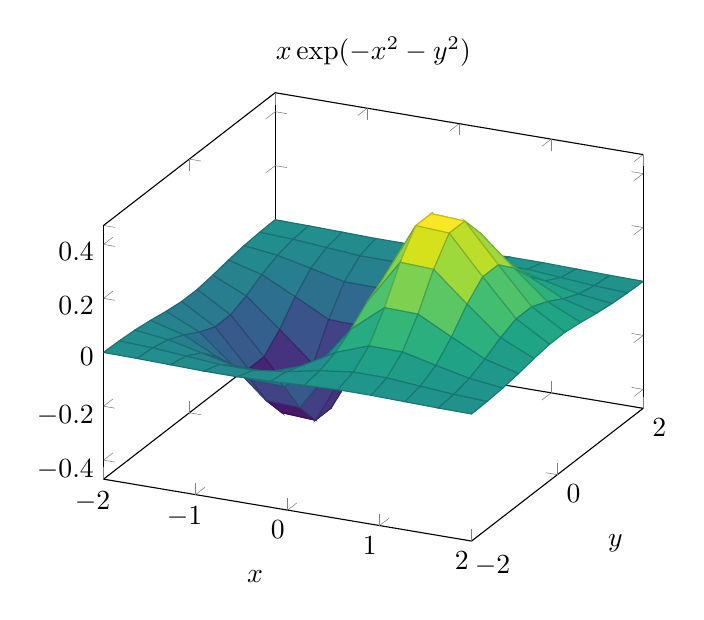
\begin{tikzpicture}
        \begin{axis}[
                title={$x \exp(-x^2-y^2)$},
                xlabel=$x$, ylabel=$y$,
                % small,
            ]
            \addplot3[
                surf,
                domain=-2:2,
                % domain y=-1:1,
                colormap/viridis,
                samples=12,
            ]
            {exp(-x^2-y^2)*x};
        \end{axis}
    \end{tikzpicture}
\end{figure}

\begin{figure}[ht]
    \centering
    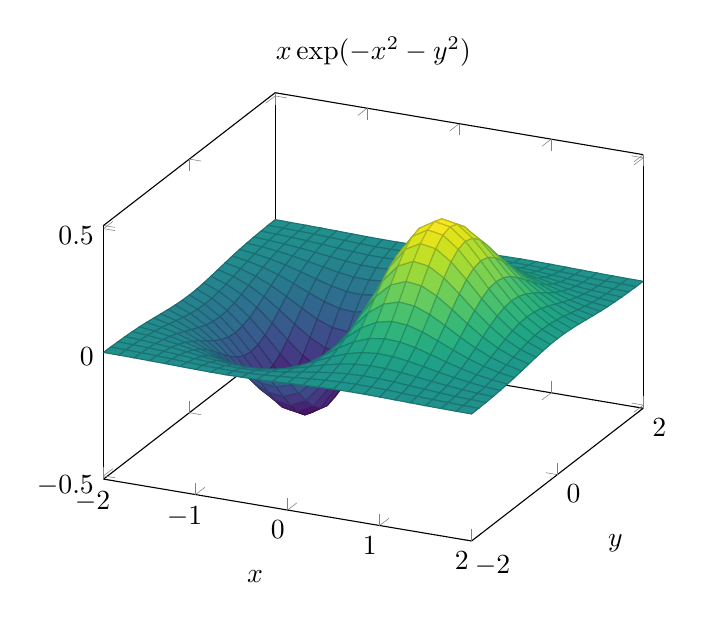
\begin{tikzpicture}
        \begin{axis}[
                title={$x \exp(-x^2-y^2)$},
                xlabel=$x$, ylabel=$y$,
                % small,
            ]
            \addplot3[
                surf,
                domain=-2:2,
                % domain y=-1:1,
                colormap/viridis,
                samples=25,
            ]
            {exp(-x^2-y^2)*x};
        \end{axis}
    \end{tikzpicture}
\end{figure}

\begin{figure}[ht]
    \centering
    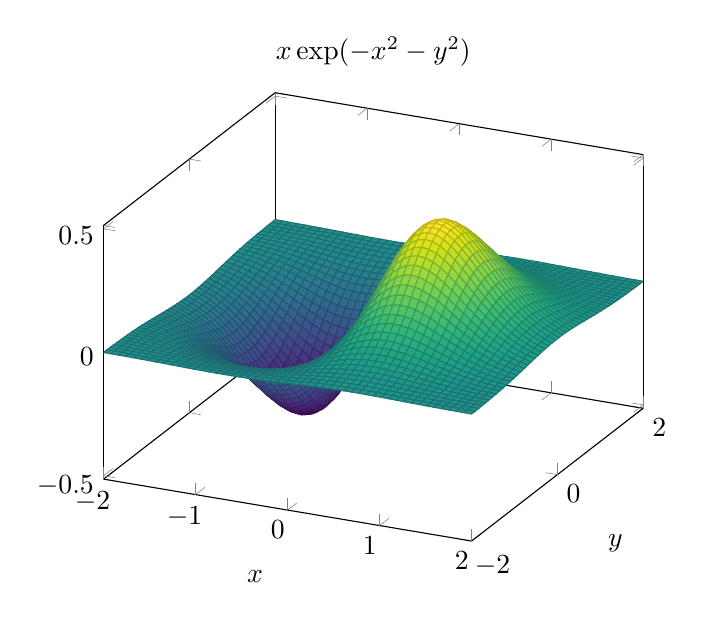
\begin{tikzpicture}
        \begin{axis}[
                title={$x \exp(-x^2-y^2)$},
                xlabel=$x$, ylabel=$y$,
                % small,
            ]
            \addplot3[
                surf,
                domain=-2:2,
                % domain y=-1:1,
                colormap/viridis,
                samples=50,
            ]
            {exp(-x^2-y^2)*x};
        \end{axis}
    \end{tikzpicture}
\end{figure}

\begin{figure}[ht]
    \centering
    \begin{tikzpicture}
        \begin{axis}[
                title={$x \exp(-x^2-y^2)$},
                xlabel=$x$, ylabel=$y$,
                % small,
            ]
            \addplot3[
                surf,
                domain=-2:2,
                % domain y=-1:1,
                colormap/viridis,
                samples=100,
            ]
            {exp(-x^2-y^2)*x};
        \end{axis}
    \end{tikzpicture}
\end{figure}

\Blinddocument

\begin{figure*}
    \centering
    \begin{tikzpicture}
        \begin{axis}[
                colormap/PuOr,
            ]
            \addplot3+ [
                mesh,
                scatter,
                samples=10,
                domain=0:1,
            ] {x*(1-x)*y*(1-y)};
        \end{axis}
    \end{tikzpicture}
\end{figure*}

\begin{figure*}
    \centering
    \begin{tikzpicture}
        \begin{axis}[
                title={$x \exp(-x^2-y^2)$},
                domain=-2:2,
                colormap/viridis,
            ]
            \addplot3 [
                contour lua={
                        contour dir=y,
                        labels=false,
                        number=60,
                    },
                thick,
            ] {exp(-x^2-y^2)*x};
        \end{axis}
    \end{tikzpicture}
\end{figure*}

\begin{figure*}
    \centering
    \tdplotsetmaincoords{60}{130}
    \begin{tikzpicture}[tdplot_main_coords]
        % The function that is rotated
        \tikzmath{function f(\x) {return 1.5 - 0.325*sin(\x r);};}
        \pgfmathsetmacro{\dominio}{2.0}
        \pgfmathsetmacro{\xi}{-\dominio}
        \pgfmathsetmacro{\step}{(\dominio-\xi)/70.0}
        \pgfmathsetmacro{\xs}{\xi+\step}
        \pgfmathsetmacro{\max}{3}
        % Circumferences (behind the coordiante axis)
        \foreach \x in {\xi,\xs,...,\dominio}{
        \pgfmathsetmacro{\radio}{f(\x)}	% radius of the circumference of the solid of revolution
        \draw[cyan,very thick,opacity=0.35] plot[domain=0.5*pi:2.0*pi,smooth,variable=\t] ({\radio*cos(\t r)},{\x},{\radio*sin(\t r});
            }
        % Part of the solid of revolution behind the coordinate axis
        \foreach \angulo in {358,356,...,90}{
                \draw[cyan,very thick,rotate around y=\angulo,opacity=0.35] plot[domain=-\dominio:\dominio,smooth,variable=\t] ({0},{\t},{f(\t)});
            }
        % Graph of the function rotated about the $y$ axis
        \draw[red,ultra thick] plot[domain=-\dominio:\dominio,smooth,variable=\t] ({0},{\t},{f(\t)}) node [above right] {$z = f(y)$};
        % Coordinate axis
        \draw[thick,->] (0,0,0) -- (0,\max,0) node [right] {$y$};
        \draw[thick,->] (0,0,0) -- (\max,0,0) node [left] {$x$};
        \draw[thick,->] (0,0,0) -- (0,0,\max) node [above] {$z$};
        % Circumferences (in front of the coordiante axis)
        \foreach \x in {\xi,\xs,...,\dominio}{
        \pgfmathsetmacro{\radio}{f(\x)}	% Radio del círculo al inicio del sólido de revolución
        \draw[cyan,very thick,opacity=0.35] plot[domain=0.0:0.5*pi,smooth,variable=\t] ({\radio*cos(\t r)},{\x},{\radio*sin(\t r});
            }
        % The solid of revolution (in front of the coordinate axis)
        \foreach \angulo in {0,2,...,89}{
                \draw[cyan,very thick,rotate around y=\angulo,opacity=0.35] plot[domain=-\dominio:\dominio,smooth,variable=\t] ({0},{\t},{f(\t)});
            }
    \end{tikzpicture}
\end{figure*}



\lipsum[10]

\begin{equation*}
    x = \frac{-b \pm \sqrt{b^2 - 4ac}}{2a}
\end{equation*}

\begin{greybox}{This is a title}
    This is some text.

    This is on a new line.

    This is on another new line.\\
    Here is an equation:

    \begin{equation*}
        x = \frac{-b \pm \sqrt{b^2 - 4ac}}{2a}
    \end{equation*}
\end{greybox}

\begin{redbox}{This is a title}
    This is some text.

    This is on a new line.

    This is on another new line.

    \begin{equation*}
        x = \frac{-b \pm \sqrt{b^2 - 4ac}}{2a}
    \end{equation*}
\end{redbox}

\begin{bluebox}{This is a title}
    This is some text.

    This is on a new line.

    This is on another new line.

    \begin{equation*}
        x = \frac{-b \pm \sqrt{b^2 - 4ac}}{2a}
    \end{equation*}
\end{bluebox}

\begin{greenbox}{This is a title}
    This is some text.

    This is on a new line.

    This is on another new line.

    \begin{equation*}
        x = \frac{-b \pm \sqrt{b^2 - 4ac}}{2a}
    \end{equation*}
\end{greenbox}

\begin{codebox}{This is a title}
    \begin{lstlisting}[language=C++]
        #include <iostream>

        int main() {
            std::cout << "Hello, World!" << std::endl;
            return 0;
        }
    \end{lstlisting}
\end{codebox}

\begin{lstlisting}[language=C++]
        #include <iostream>

        int main() {
            std::cout << "Hello, World!" << std::endl;
            return 0;
        }
\end{lstlisting}

\begin{theorem}
    \textbf{Pythagoras' Theorem}

    For a right triangle with legs $a$ and $b$, the length of the hypotenuse is
    $c = \sqrt{a^2 + b^2}$.

    \begin{equation*}
        a^2 + b^2 = c^2
    \end{equation*}
\end{theorem}

\begin{lemma}
    \textbf{Pythagoras' Theorem}

    For a right triangle with legs $a$ and $b$, the length of the hypotenuse is
    $c = \sqrt{a^2 + b^2}$.

    \begin{equation*}
        a^2 + b^2 = c^2
    \end{equation*}
\end{lemma}

\begin{corollary}
    \textbf{Pythagoras' Theorem}

    For a right triangle with legs $a$ and $b$, the length of the hypotenuse is
    $c = \sqrt{a^2 + b^2}$.

    \begin{equation*}
        a^2 + b^2 = c^2
    \end{equation*}
\end{corollary}

\begin{proposition}
    \textbf{Pythagoras' Theorem}

    For a right triangle with legs $a$ and $b$, the length of the hypotenuse is
    $c = \sqrt{a^2 + b^2}$.

    \begin{equation*}
        a^2 + b^2 = c^2
    \end{equation*}
\end{proposition}

This shouldn't impact the compile times. Does it??

This might work now.

This should not impact the compile times whatsoever. It should compile nice and
fast because we have Tikz externalize enabled. \LaTeX is so cool!
